%%==================================================
%% chapter3.tex for BIT Master Thesis
%% version: 0.1
%% last update: Nov 8th, 2017
%%==================================================
\chapter{半参数自适应估计与控制算法}
\label{chap:3}

\section{问题描述}

\section{超限学习机}

人工智能的发展一直推动着神经网络的研究,特别是2012年之后,深度学习(Deep Learning, DL)在图像分类、语音识别、自然语言处理等应用领域中获得了巨大成功\upcite{ZhengChenZhang2014}。目前大部分的深度学习算法大部分是基于神经网络建立。对于深度学习来说,隐含层的数量级为十几层到几百层不等,甚至上千层。深层网络结构和特征学习思想是深度学习的两大主要特点。与深度学习相比,超限学习机在不丢失精度的条件下具有快速的优势,比较见图\ref{fig:elm-dl}所示。

\begin{figure}
 \centering
 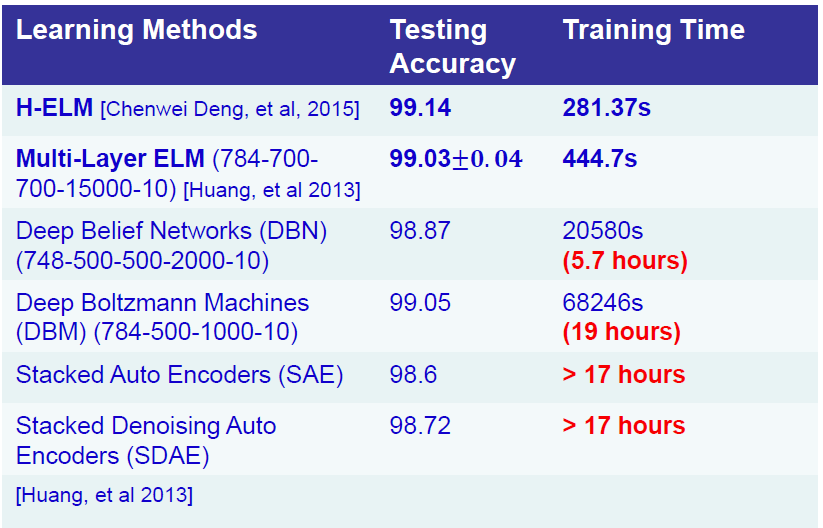
\includegraphics[width=0.7\textwidth]{figures/elm-dl}
 \caption{超限学习机与常见深度学习性能比较}\label{fig:elm-dl}
\end{figure}